\section{Simulation}\label{sec:sim}
	We conduct a simulation that uses a team of six UGVs to localize three moving targets.
	Every UGV maintains three individual PDFs, each corresponding to a target.
	At each time step, a UGV's sensor can measurement the positions of three targets.
	We assume that the UGVs know the association between the measurement and the corresponding target.
	The targets have different motion models, including the linear motion (target a), sinusoidal motion (target b), and circular motion (target c).
	Three of the UGVs have range-only sensors and the other three UGVs have bearing-only sensors.
	The interaction topology of the UGVs is time-varying and consists of four types, as shown in \Cref{fig:com_topo1}.
	A randomly generated sequence of topologies is used (\Cref{}).
	It can be noticed that, the interaction topology is \fc when all four types appears repeatedly.
	Ten layouts of the initial positions of UGVs and targets are randomly generated.
	We compare \proto-DBF with CbDF and CF.
	
	\Cref{fig:mov_sen_mov_tar1} show the simulation results of a specific layout.
	The sum of the $1^\text{st}$ UGV's individual PDFs are shown in the figures.
	\Cref{fig:step5,fig:step20,fig:step30,fig:step40} show that the \proto-DBF can successfully localize and track moving target's positions and effectively reduce the estimation uncertainty, which is similar to the performance of the CF (\Cref{fig:CF}).
	On the contrary, CbDF is less effective to reduce the estimation uncertainty.
	
	We compares the three filters in terms of the estimation error and entropy of the uncertainty.
	The estimation error is defined as the difference between the true target position and the MAP estimate of the individual PDF:
	\begin{equation*}
		\Delta_k = \|x^\text{MAP}_k-x^g_k\|_2.
	\end{equation*}
	The entropy of the uncertainty is
	\begin{equation*}
		H_k = \sum\limits_{X_k\in S} -P_{pdf}(X_k)\log(P_{pdf}(X_k)).
	\end{equation*}
	The average of the estimation error and entropy across ten layouts are shown in \Cref{fig:metrics}.
	For \proto-DBF, we only show the results of the $1^\text{st}$, $3^\text{rd}$, and $5\thi$ UGV for the clarity of the plots.
	It can be noticed that, CF achieves the most accurate position estimation and fastest entropy reduction. 
	This is expected result since the CF utilizes all sensor measurements.
	The \proto-DBF achieves similar results as the CF asymptotically. 
	This is a very interesting results, since \proto-DBF only communicates with neighboring UGVs and have a subset of other UGVs' measurements.
	The CbDF achieves similar position estimation performance and the CF and \proto-DBF. 
	However, it fails to effectively reduce the estimation entropy.
	A quantitative comparison is shown in \Cref{Table}.

	\todohere{add a table for quantitative comparison.}
		
	\begin{figure}%[thpb]
		\centering
		\begin{subfigure}[b]{0.3\textwidth}
			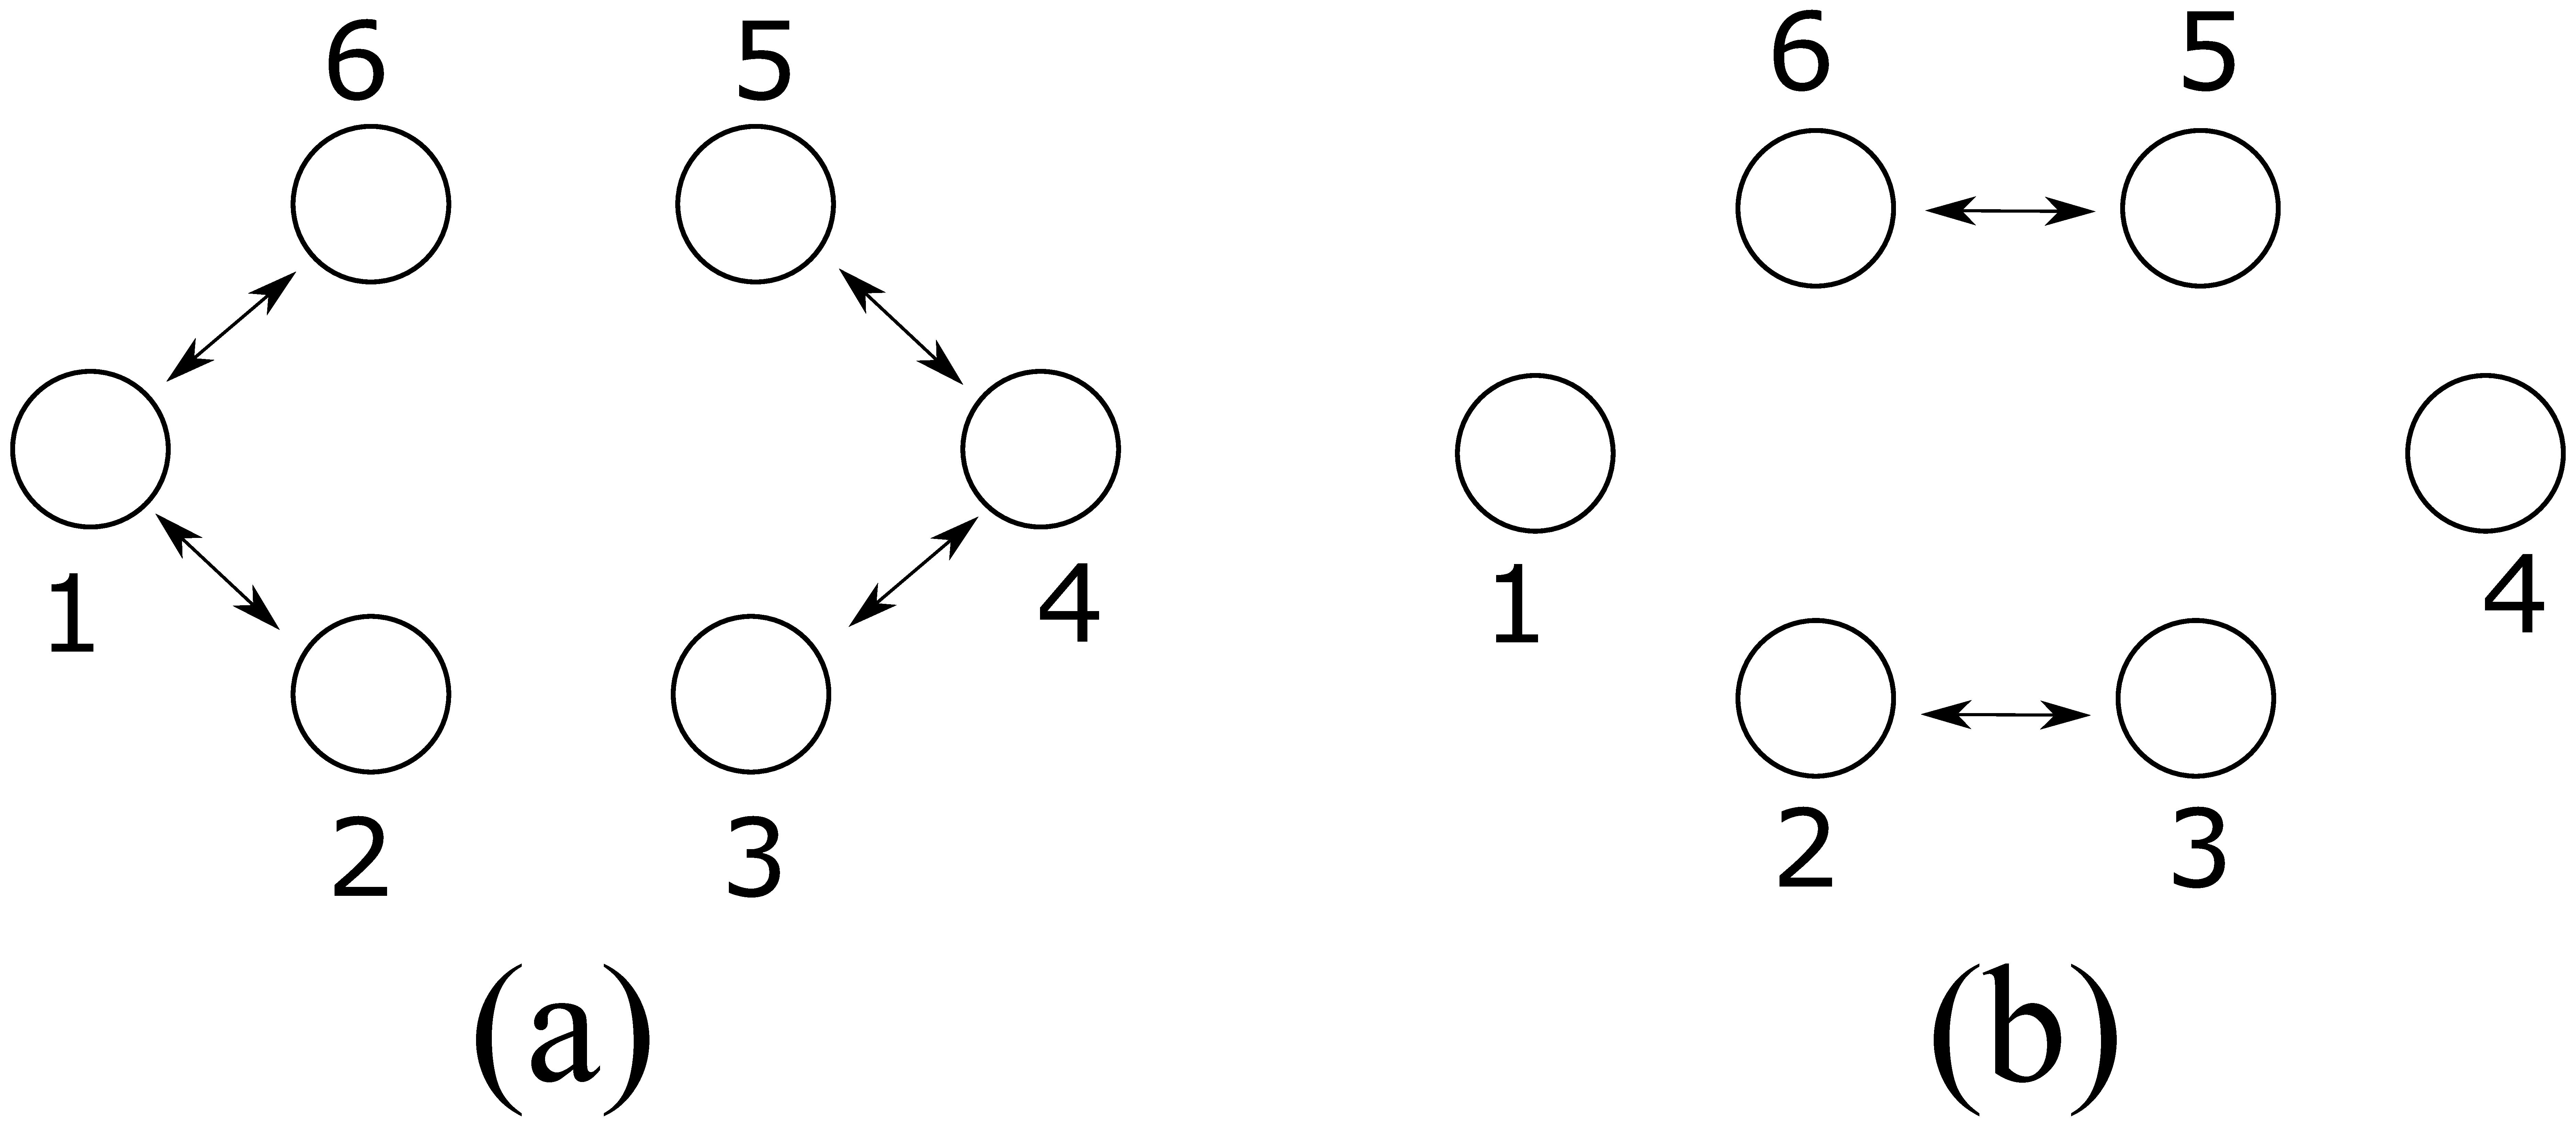
\includegraphics[width=\textwidth]{figures/com_topo1}
			\caption{Collection of changing topologies}\label{fig:com_topo1}
		\end{subfigure}
		~
		\begin{subfigure}[b]{0.23\textwidth}
			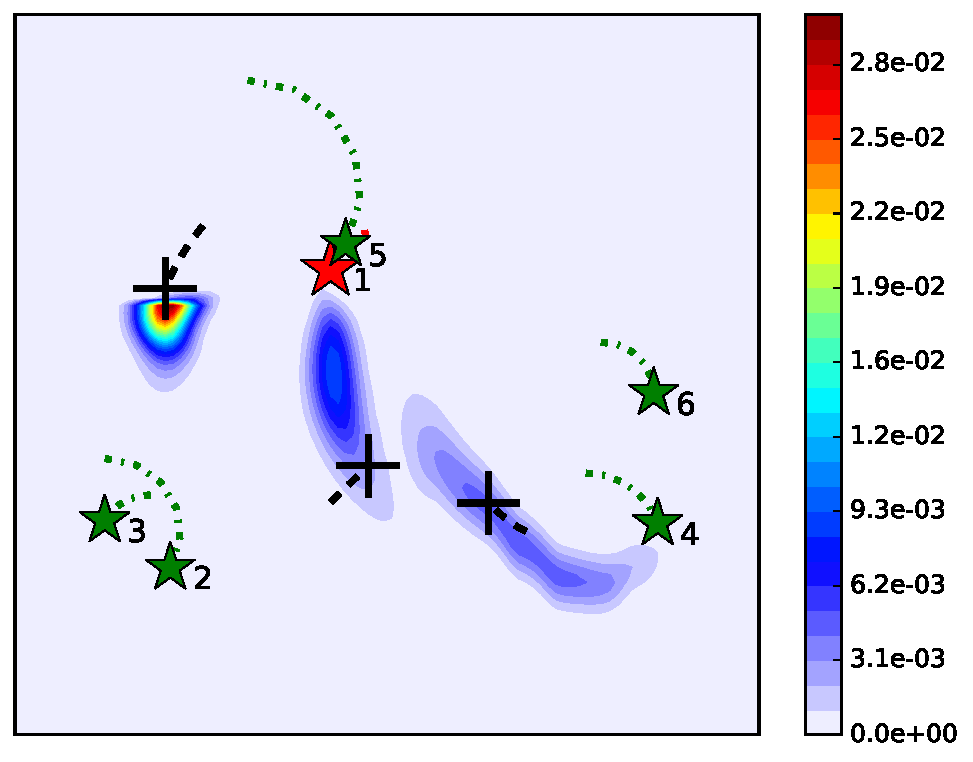
\includegraphics[width=\textwidth]{figures/hetero_mov_sen_mov_tar_rbt1_step5}
			\caption{\proto-DBF Step 5}\label{fig:step5}
		\end{subfigure}
		\begin{subfigure}[b]{0.23\textwidth}
			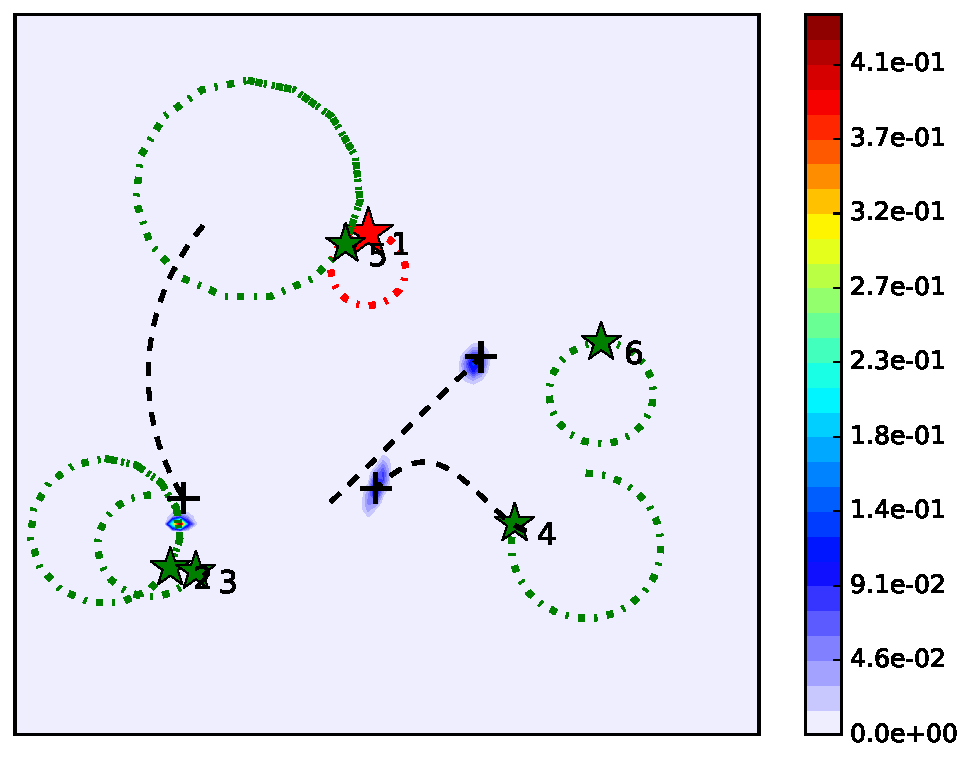
\includegraphics[width=\textwidth]{figures/hetero_mov_sen_mov_tar_rbt1_step20}
			\caption{\proto-DBF Step 20}\label{fig:step20}
		\end{subfigure}
		\begin{subfigure}[b]{0.23\textwidth}
			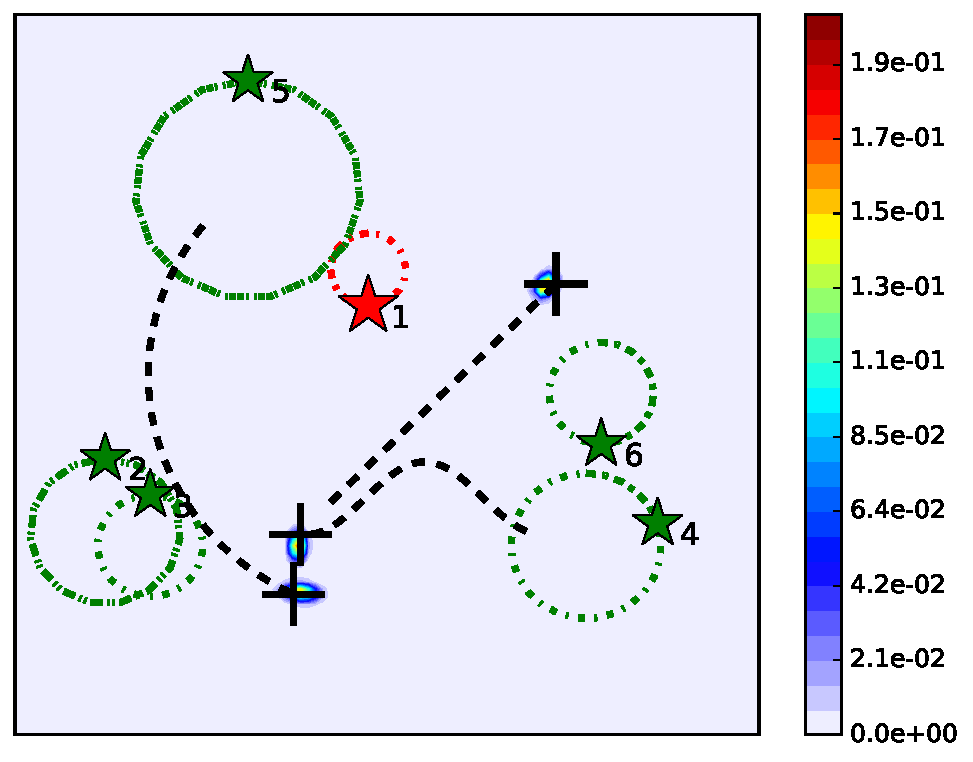
\includegraphics[width=\textwidth]{figures/hetero_mov_sen_mov_tar_rbt1_step30}
			\caption{\proto-DBF Step 30}\label{fig:step30}
		\end{subfigure}
		\begin{subfigure}[b]{0.23\textwidth}
			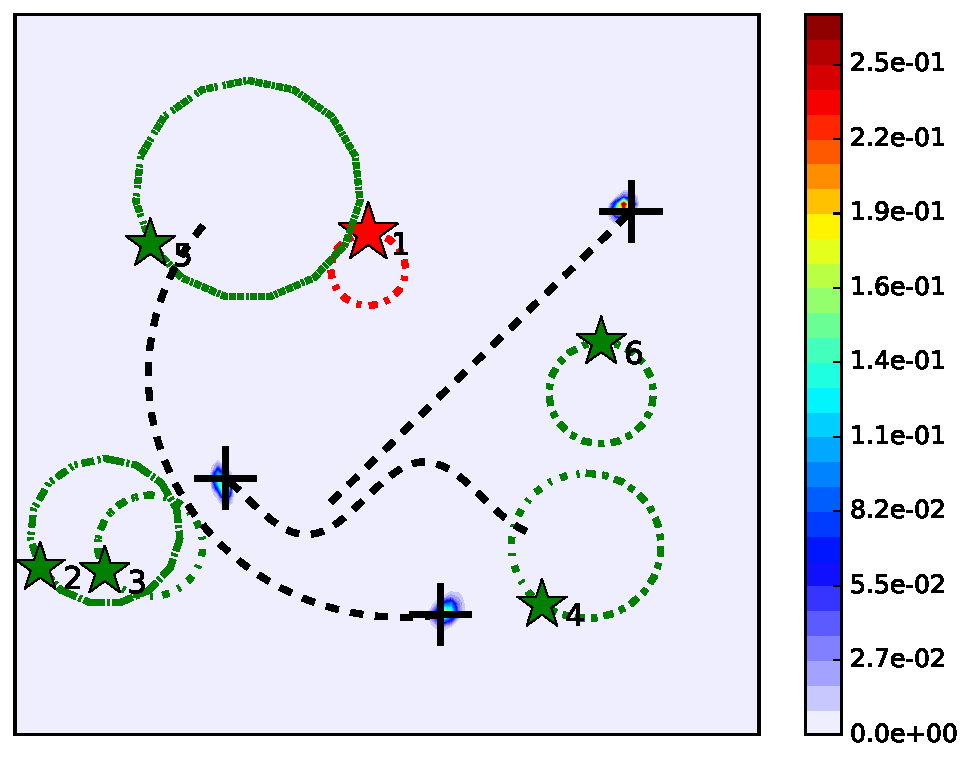
\includegraphics[width=\textwidth]{figures/hetero_mov_sen_mov_tar_rbt1_step40}
			\caption{\proto-DBF Step 40}\label{fig:step40}
		\end{subfigure}	
%		\begin{subfigure}[b]{0.23\textwidth}
%			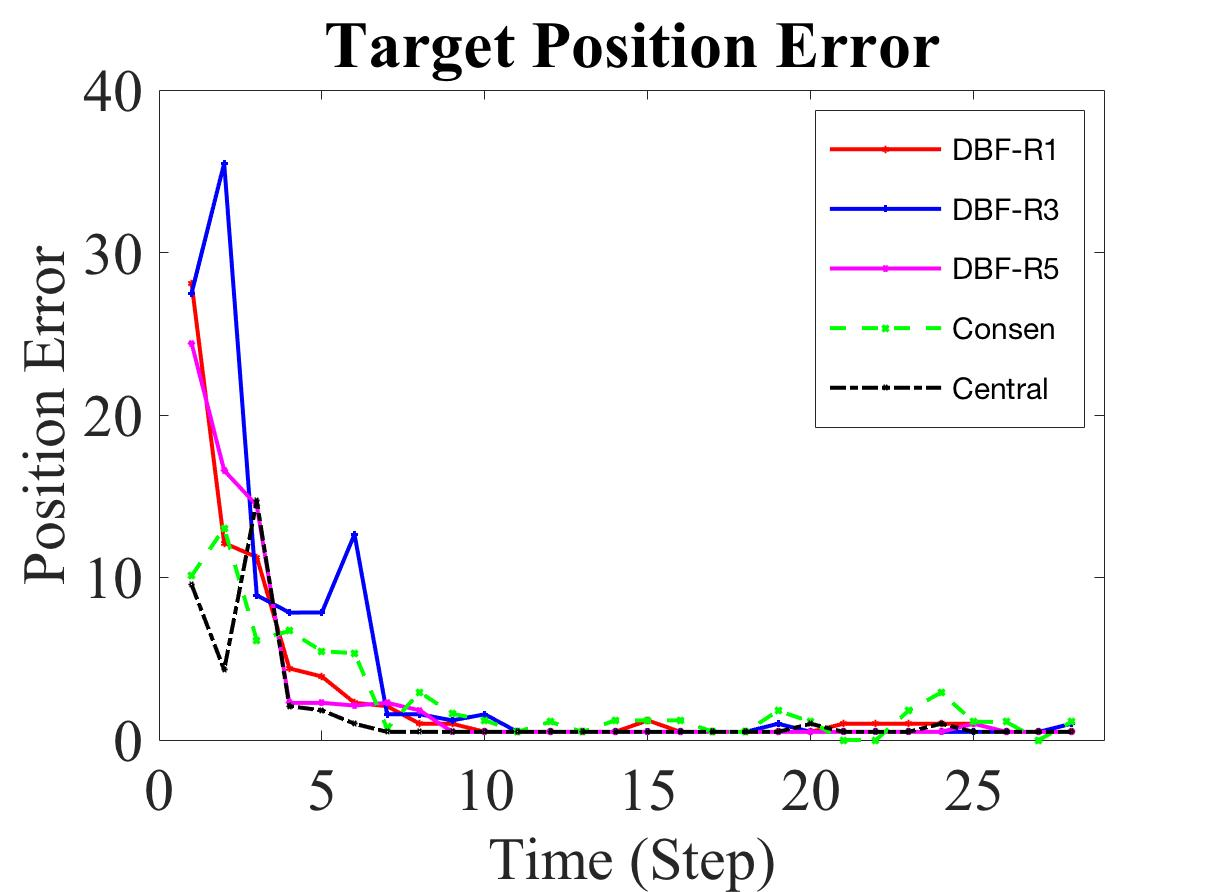
\includegraphics[width=\textwidth]{figures/trial_pos_err}
%			\caption{Consensus Filter}\label{fig:CbDF}
%		\end{subfigure}	
%		\begin{subfigure}[b]{0.23\textwidth}
%			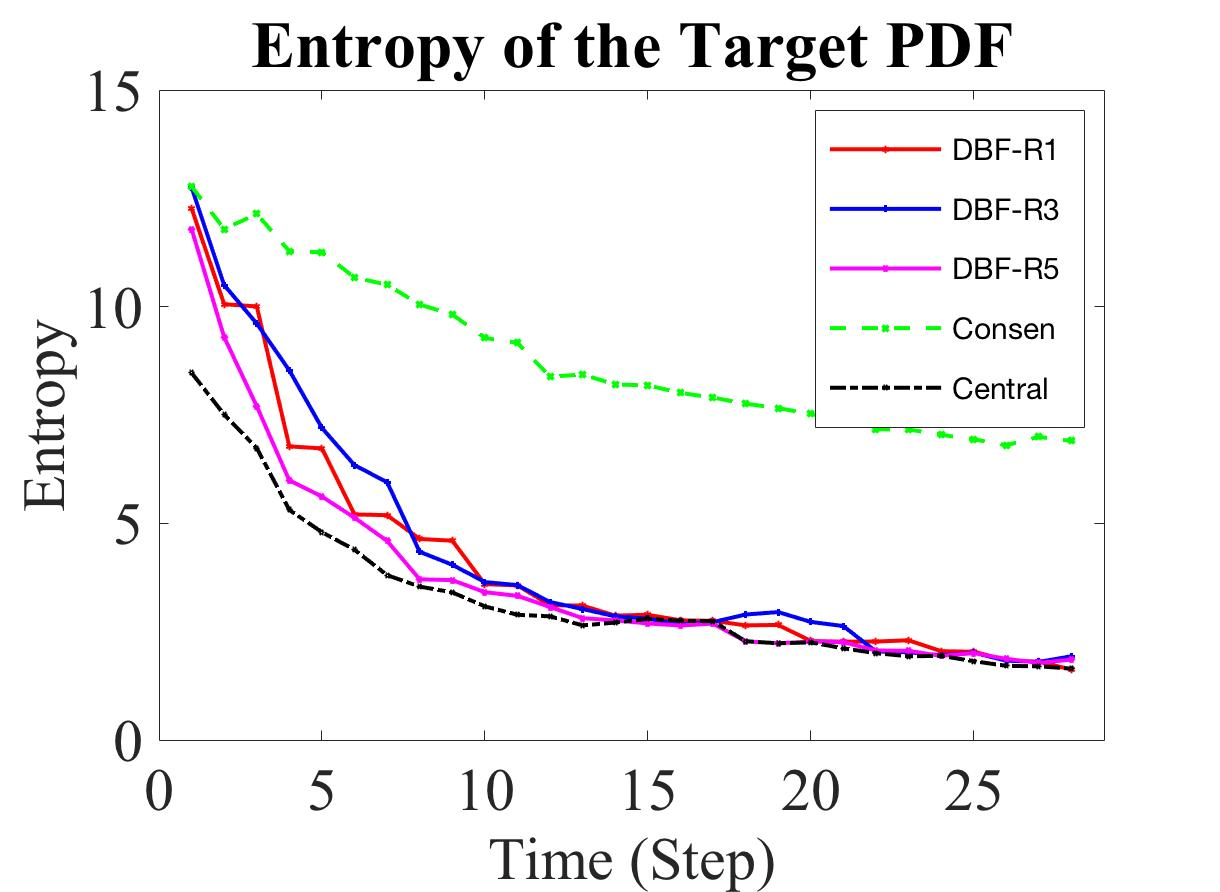
\includegraphics[width=\textwidth]{figures/trial_ent_err}
%			\caption{Centralized Filter}\label{fig:CF
%		\end{subfigure}		
		\caption{First scenario: (a) two types of topologies; (b) individual PDF of the $3^\text{rd}$ UGV after initial observation; (c)-(e) PDFs at the end of simulation using different filters; (f) average position estimation errors; (g) average entropy of PDF. In last two figures, metrics are based on the PDFs of the $1^\text{st}$, $3^\text{rd}$ and $5\thi$ UGV using \proto-DBF, the common PDF using CbDF and using CF.\todonote{add step 40 plot of ConF and CF.}}
		\label{fig:mov_sen_mov_tar1}
%		\vspace{-1.3em}
	\end{figure}
	
	\begin{figure}%[thpb]
		\centering
		\begin{subfigure}[b]{0.23\textwidth}
			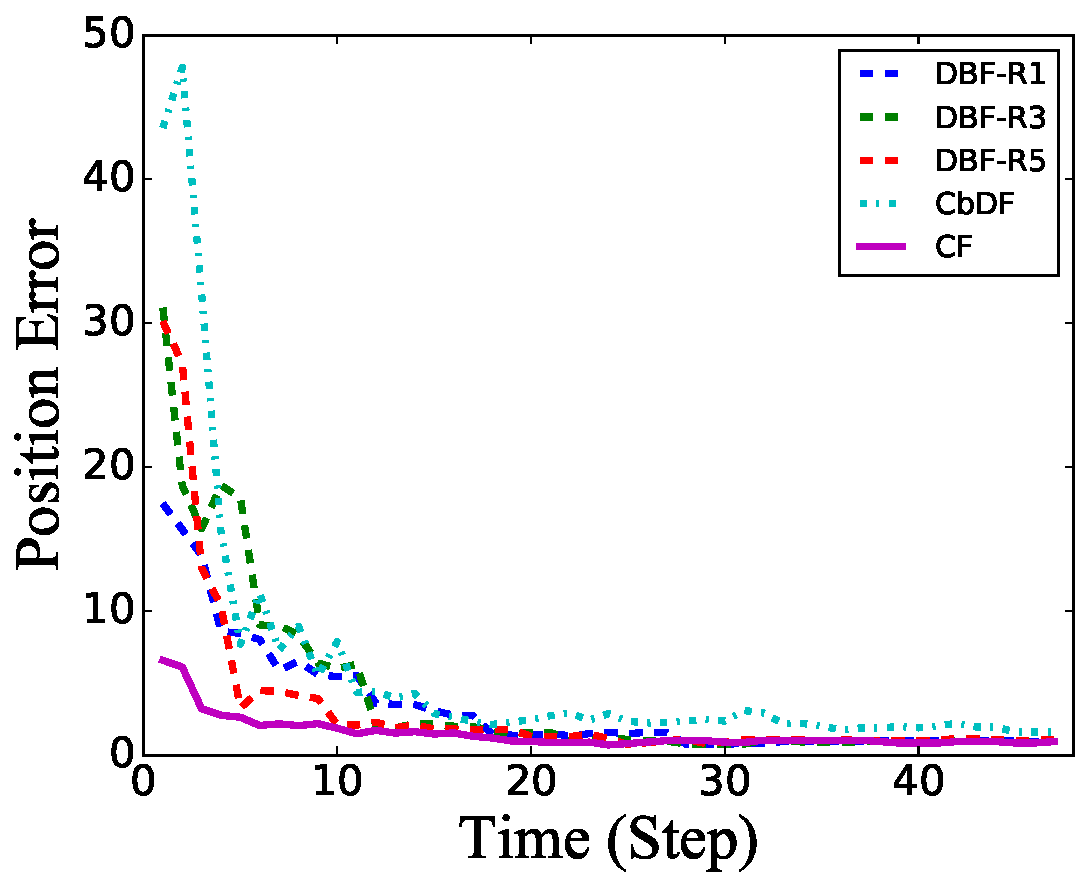
\includegraphics[width=\textwidth]{figures/hetero_mov_sen_mov_tar_pos_err_noise_linear}
			\caption{Position Error of Target $1$}\label{fig:lin_pos_err}
		\end{subfigure}				
		\begin{subfigure}[b]{0.23\textwidth}
			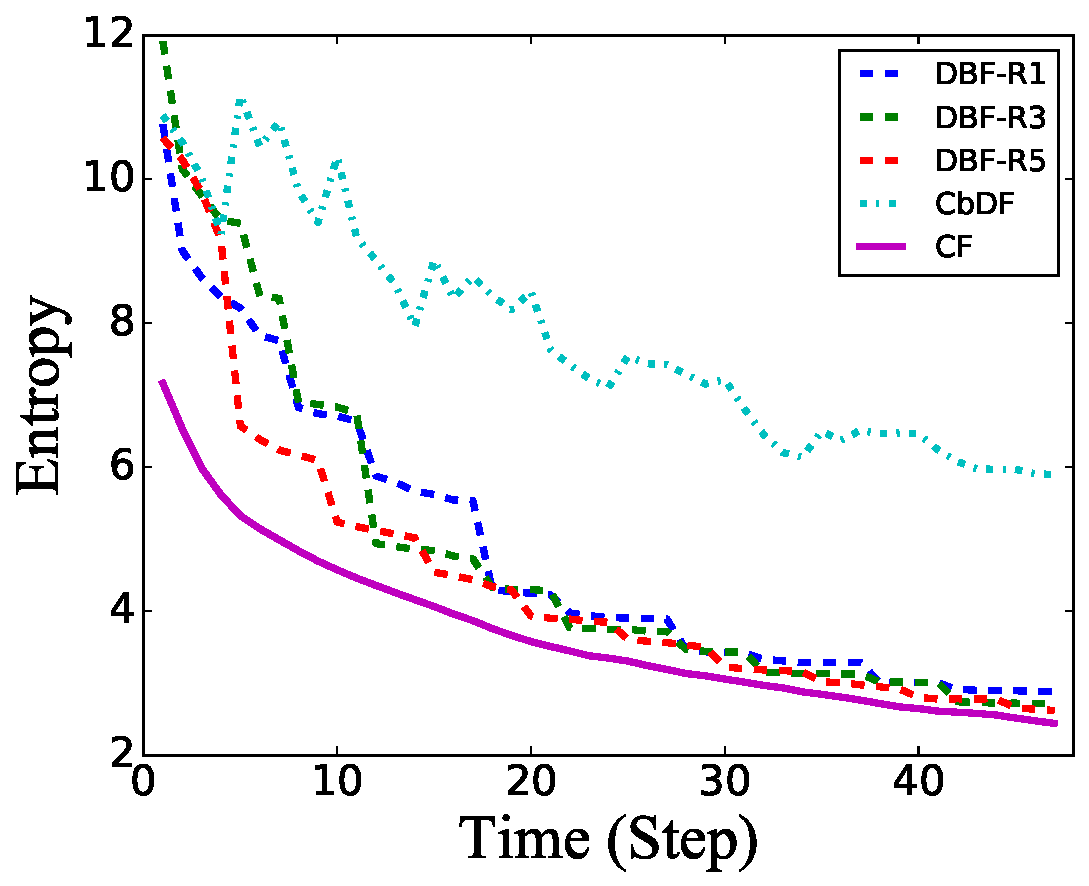
\includegraphics[width=\textwidth]{figures/hetero_mov_sen_mov_tar_entropy_noise_linear}
			\caption{Entropy of Target $1$}\label{fig:lin_ent}
		\end{subfigure}	
		\begin{subfigure}[b]{0.23\textwidth}
			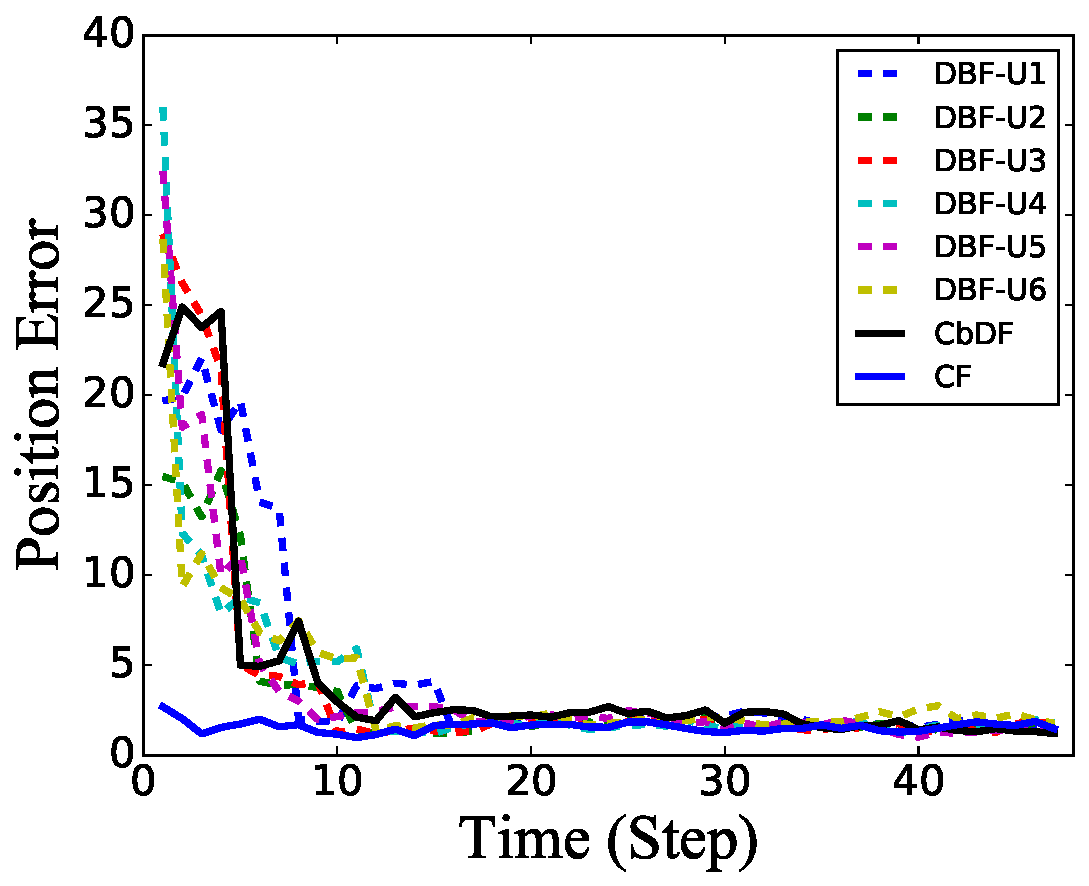
\includegraphics[width=\textwidth]{figures/hetero_mov_sen_mov_tar_pos_err_noise_circle}
			\caption{Position Error of Target $2$}\label{fig:cir_pos_err}
		\end{subfigure}
		\begin{subfigure}[b]{0.23\textwidth}
			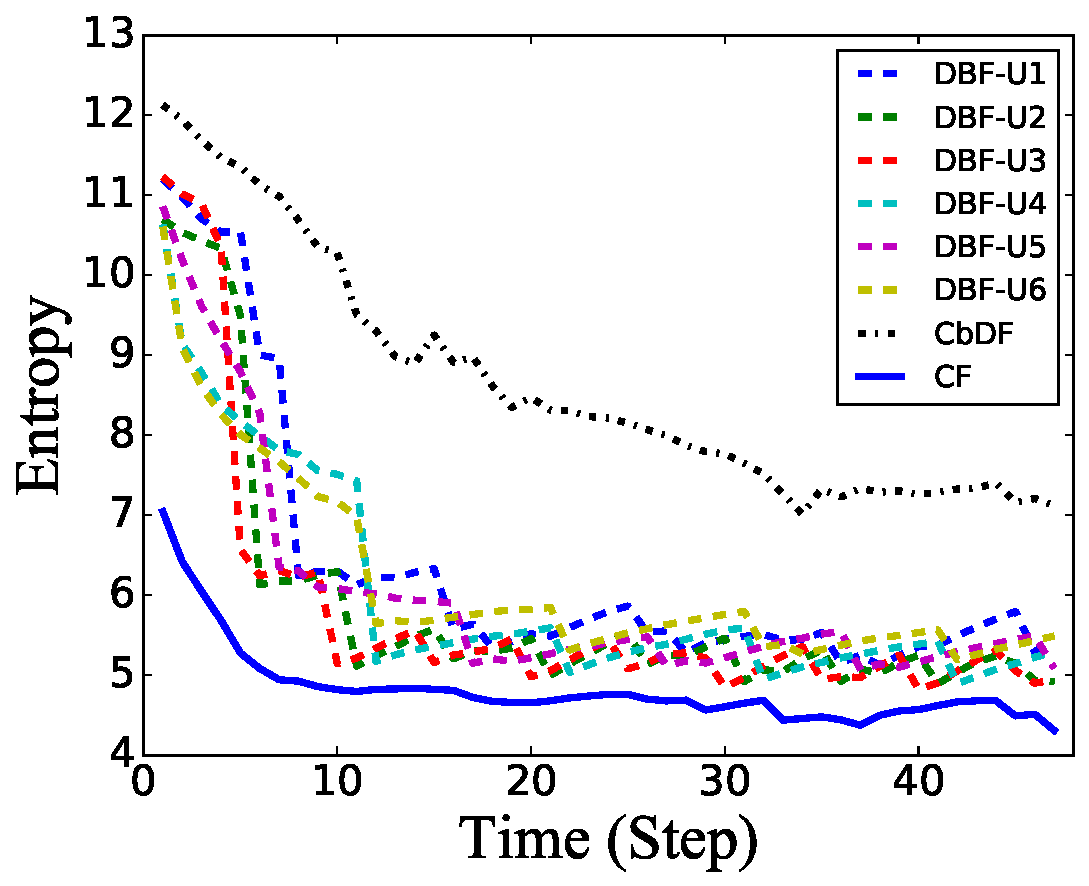
\includegraphics[width=\textwidth]{figures/hetero_mov_sen_mov_tar_entropy_noise_circle}
			\caption{Entropy of Target $2$}\label{fig:cir_ent}
		\end{subfigure}			
		\begin{subfigure}[b]{0.23\textwidth}
			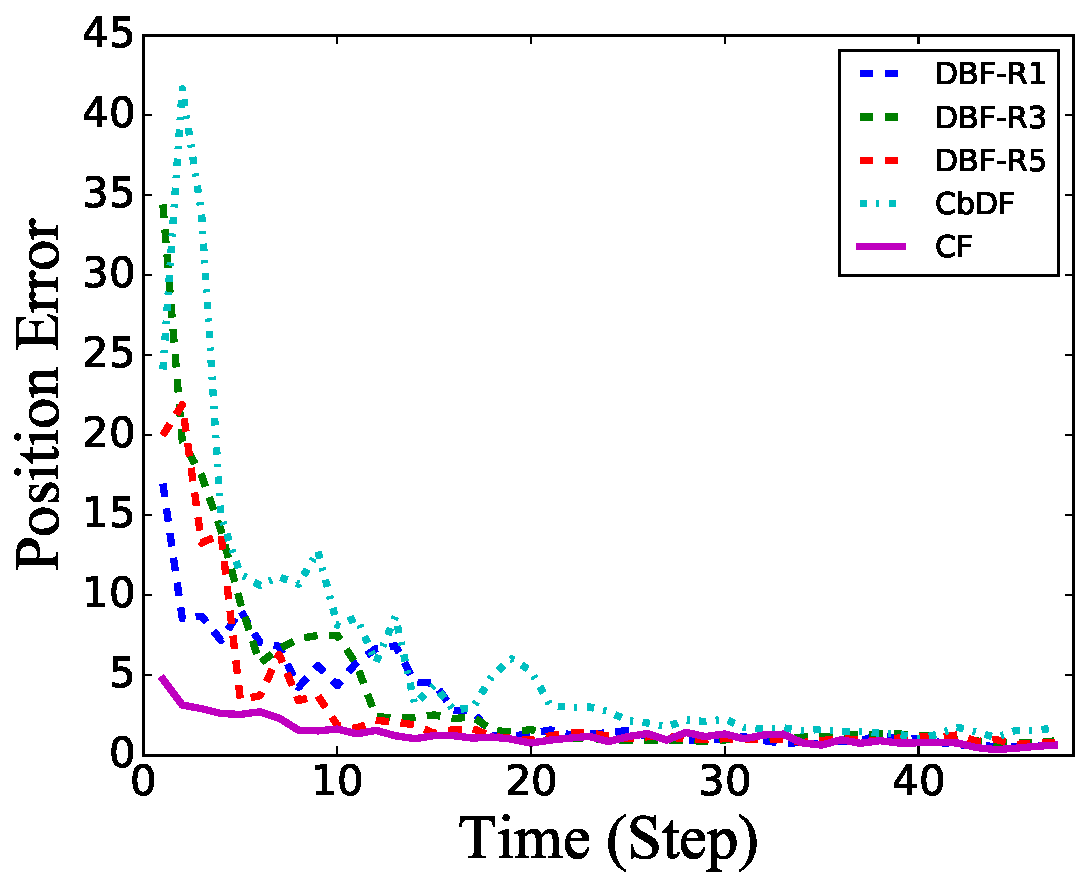
\includegraphics[width=\textwidth]{figures/hetero_mov_sen_mov_tar_pos_err_noise_sin}
			\caption{Position Error of Target $3$}\label{fig:sin_pos_err}
		\end{subfigure}
		\begin{subfigure}[b]{0.23\textwidth}
			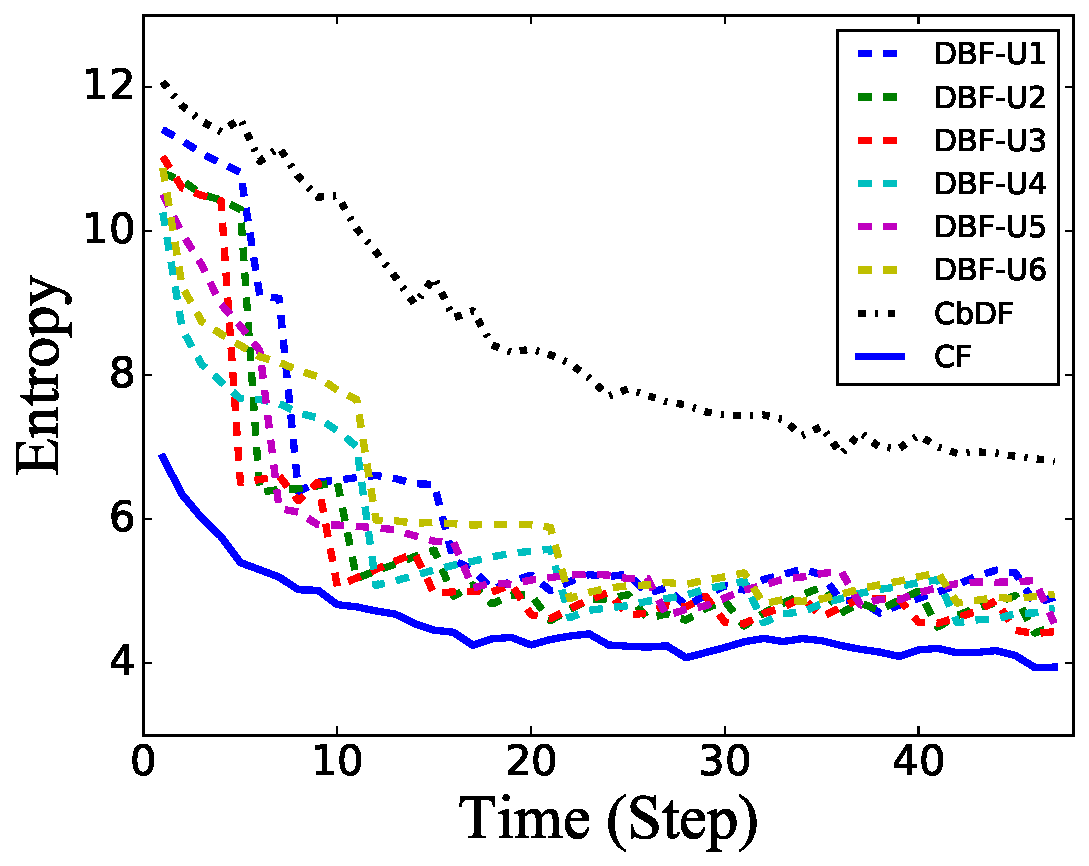
\includegraphics[width=\textwidth]{figures/hetero_mov_sen_mov_tar_entropy_noise_sin}
			\caption{Entropy of Target $3$}\label{fig:sin_ent}
		\end{subfigure}		
		\caption{First scenario: (a) two types of topologies; (b) individual PDF of the $3^\text{rd}$ UGV after initial observation; (c)-(e) PDFs at the end of simulation using different filters; (f) average position estimation errors; (g) average entropy of PDF. In last two figures, metrics are based on the PDFs of the $1^\text{st}$, $3^\text{rd}$ and $5\thi$ UGV using \proto-DBF, the common PDF using CbDF and using CF.}
		\label{fig:metrics}
		%		\vspace{-1.3em}
	\end{figure}
	
%	This section simulates two sets of dynamically changing interaction topologies to demonstrate the effectiveness of \proto-DBF.
%	Each scenario includes six static UGVs, represented as the square and stars in \cref{fig:sta_sen_sta_tar1} and \cref{fig:sta_sen_sta_tar2}.
%	The square represents the UGV whose individual PDF is shown in the figures.
%	UGVs are equipped with range-only sensors with zero-mean Gaussian white noise.
%%	 and the sensor model, \cref{eqn:bin_sensor1,eqn:bin_sensor0}, takes the form of Gaussian functions \cite{bonnie2012modelling}:
%%	%\small\begin{align}\label{eqn:gauss_sensor}
%%	\small\begin{subequations}\label{eqn:gauss_sensor}
%%		\begin{align}
%%			P(z^i_k=1|x^T;x^{R,i})&=e^{-\frac{1}{2}(x^T-x^{R,i})^T{\Sigma}^{-1}(x^T-x^{R,i})},\\
%%			%		\exp\left\lbrace -\frac{1}{2}(x^T-x^R)^T{\Sigma}^{-1}(x^T-x^R)\right\rbrace \\
%%			P(z^i_k=0|x^T;x^{R,i})&=1-P(z^i_k=1|x^T;x^{R,i}).
%%		\end{align}
%%	\end{subequations}\normalsize
%	%\end{align}\normalsize
%	%where $x^s$ denotes the UGV position where current observation is obtained. 
%	%Figure 4 shows the 1-D illustration of Gaussian binary sensor model.
%	%where $x^R$ denotes the UGV position, which is included in UGV state $y^R$.
%	
%	\cref{fig:com_topo1} and \cref{fig:com_topo2} illustrate the collections of changing interaction topologies for the first and second scenario, respectively, one with two topologies and the other with three topologies.
%	The union of topologies in each collection is designed to be jointly connected.
%	In both scenarios, topologies appear alternatively such that their union are connected frequently enough.
%
%	In both scenarios, \proto-DBF is compared with two commonly adopted approaches in multi-agent filtering: the consensus-based distributed filtering (CbDF) method and the centralized filtering (CF) method.
%	The CbDF requires robots to continually exchange their individual PDFs with direct neighbors, using the average of all received and its own individual PDFs as the updated individual PDF.
%	Multiple rounds of communication and averaging are conducted at each time step to ensure the convergence of each robot's individual PDF.
%	The CF assumes a central unit that can constantly receive and fuse all robots' latest observations into a single PDF.
%	10 test trials with randomly generated initial target positions are run and each trial is terminated after 150 time steps.
%	The average error between the estimated and true target position and the average entropy of individual PDFs of all 10 trials are compared among these three approaches.
%	
%	\begin{figure}%[thpb]
%		\centering
%		\begin{subfigure}[b]{0.3\textwidth}
%			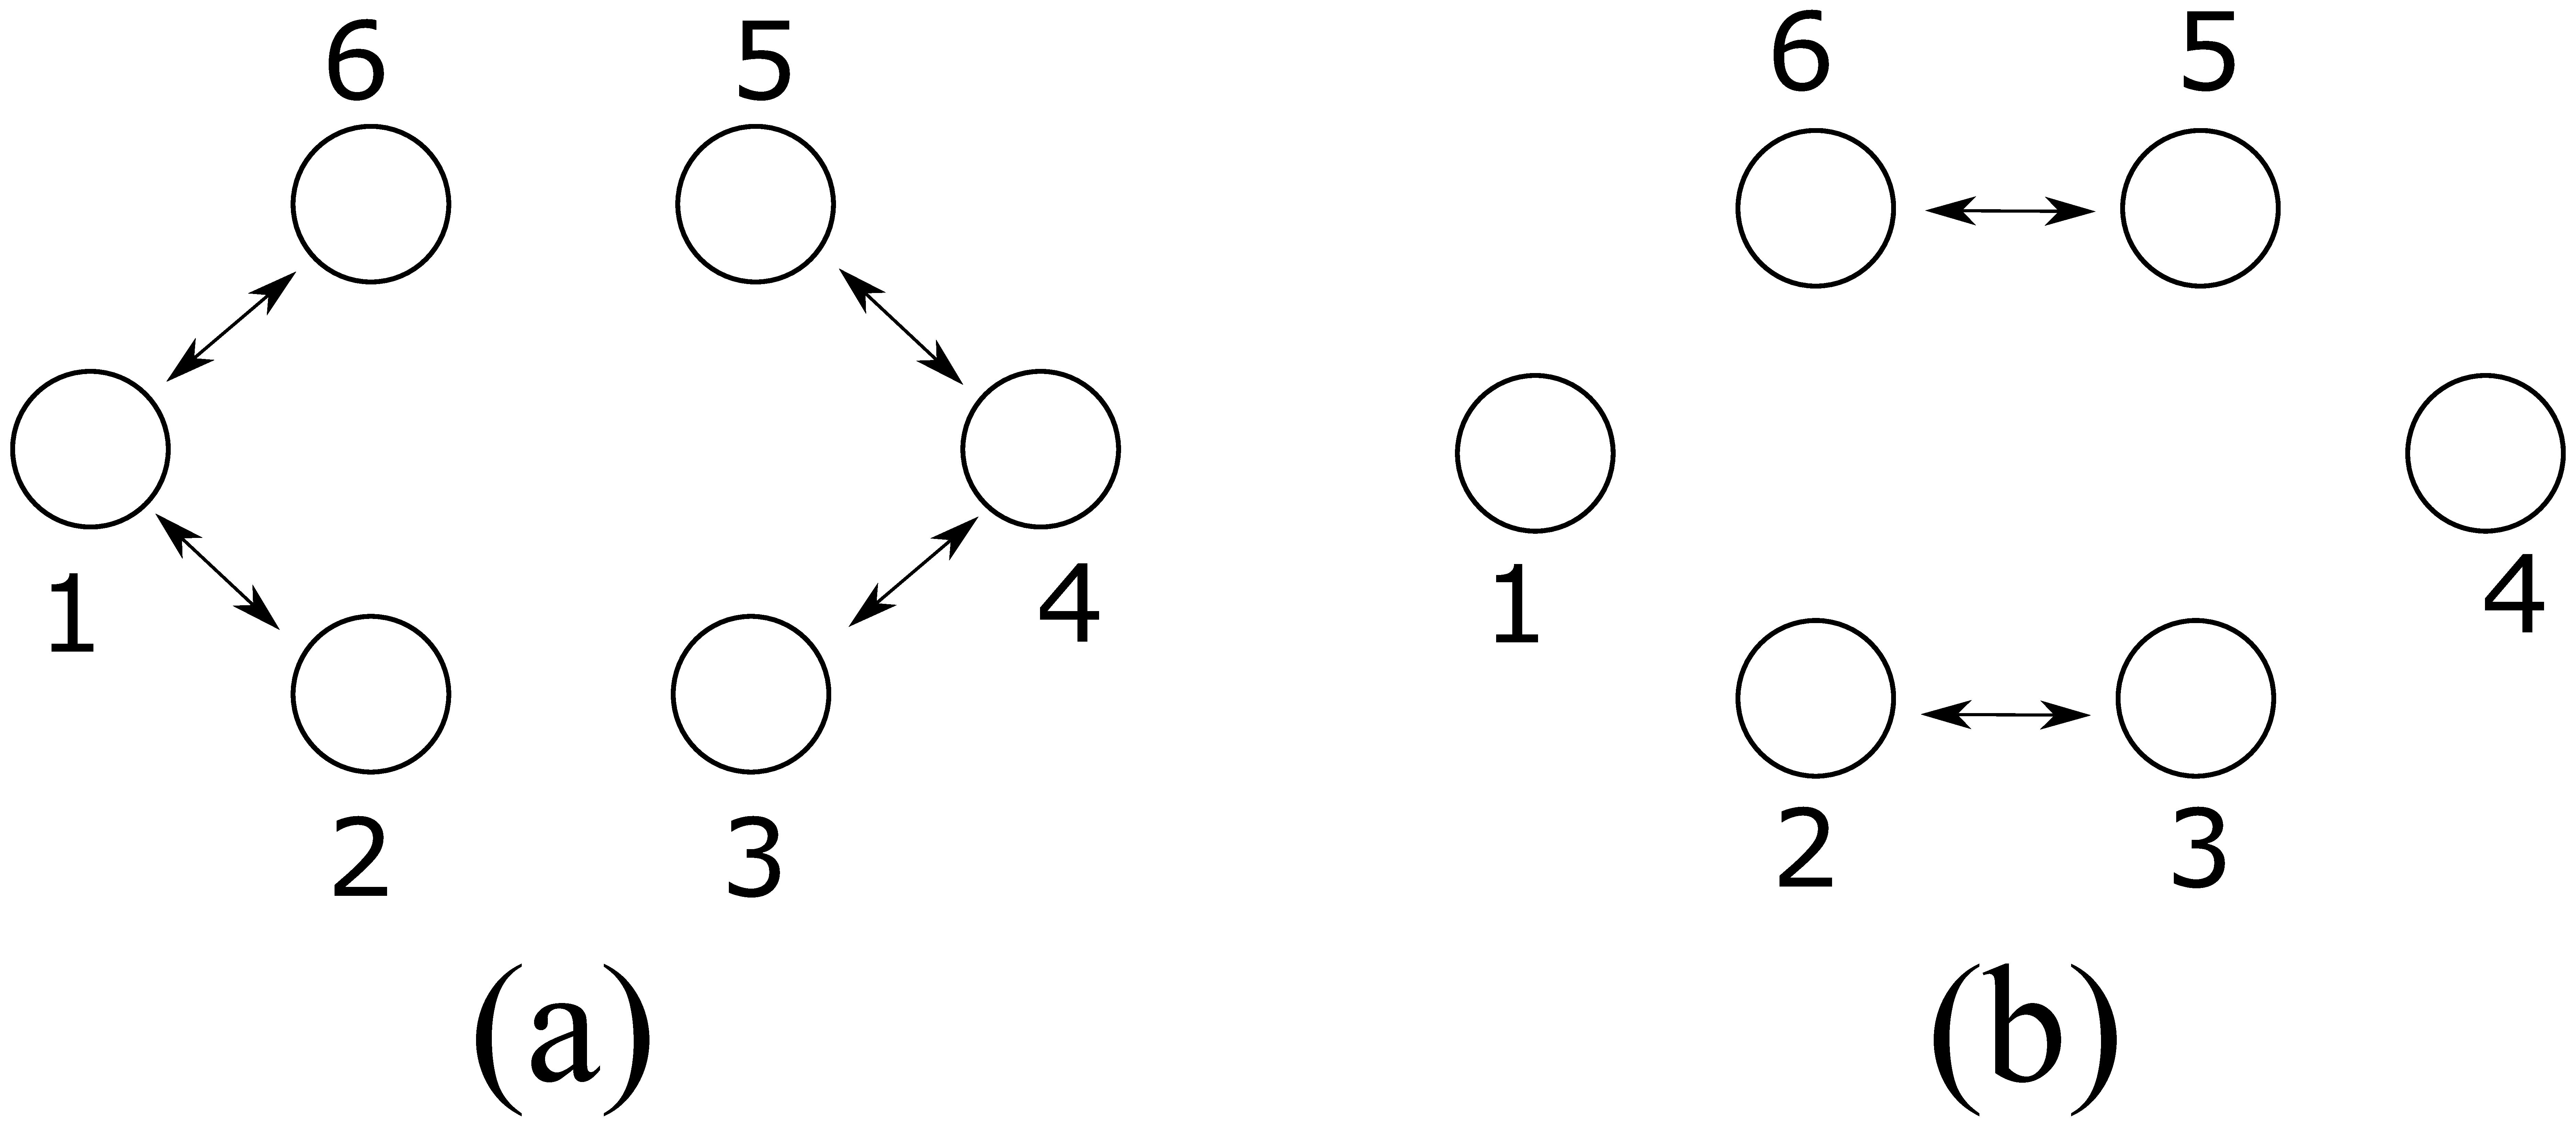
\includegraphics[width=\textwidth]{figures/com_topo1}
%			\caption{Collection of changing topologies}\label{fig:com_topo1}
%		\end{subfigure}
%		~
%		\begin{subfigure}[b]{0.21\textwidth}
%			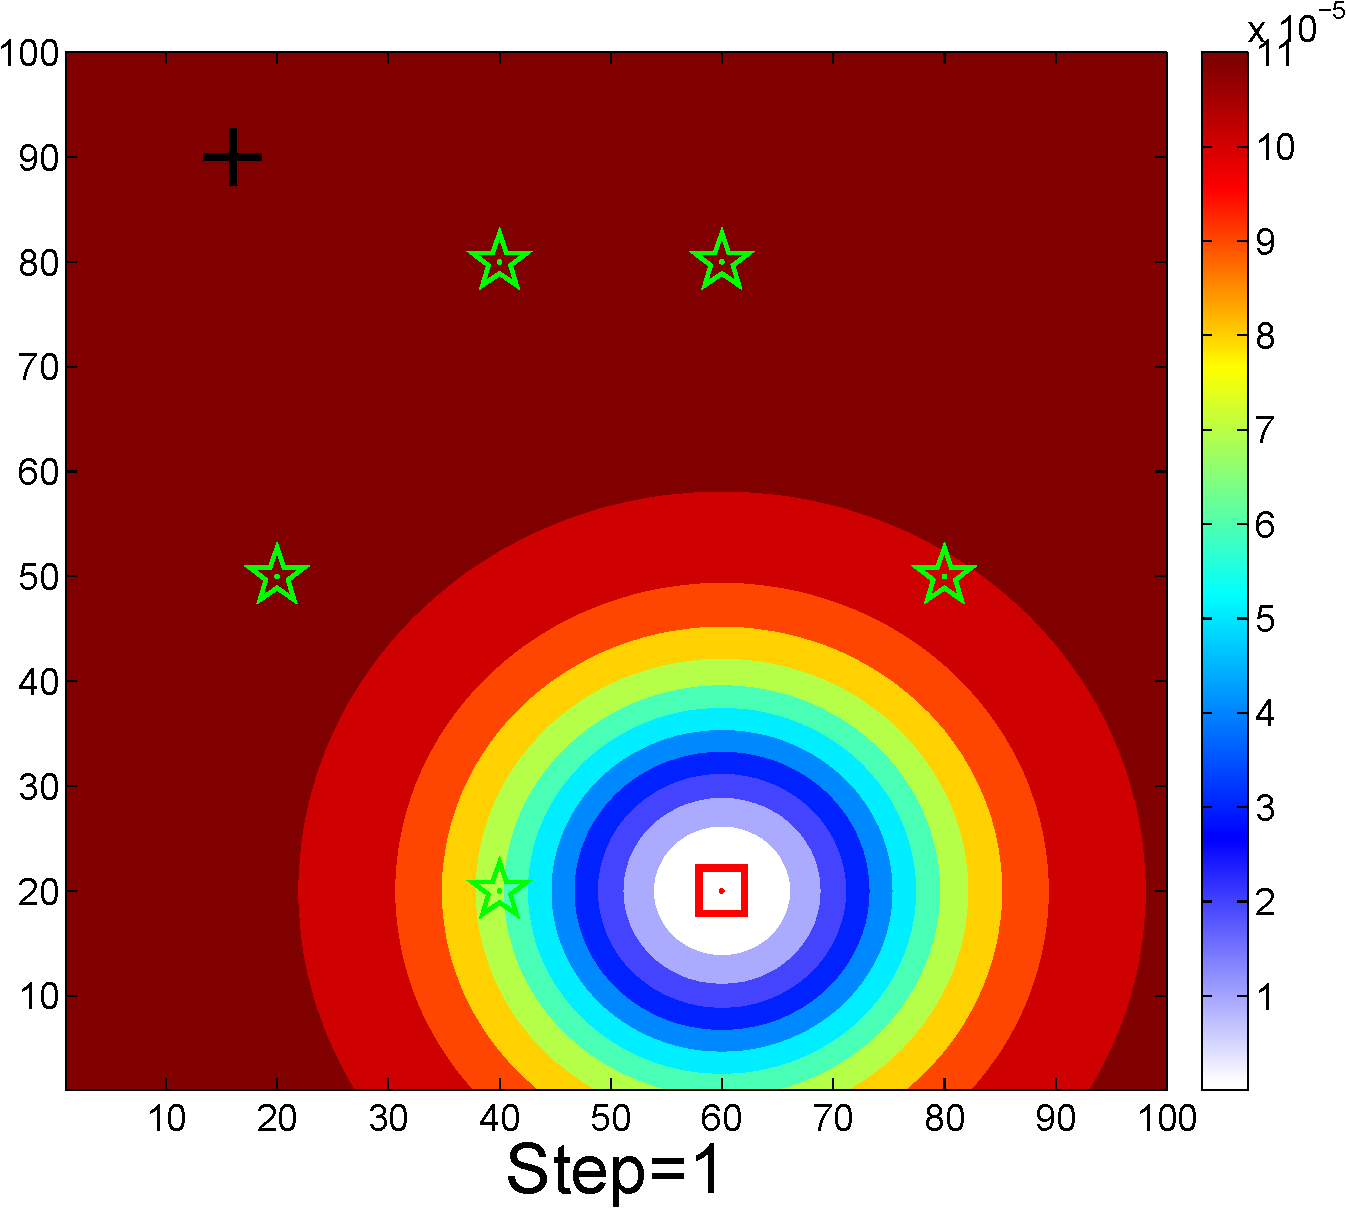
\includegraphics[width=\textwidth]{figures/sta_sen_sta_tar_top1_3_dbf_first}
%			\caption{Individual PDF}\label{fig:sta_sen_sta_tar_top1_init_dbf}
%		\end{subfigure}
%		\begin{subfigure}[b]{0.21\textwidth}
%			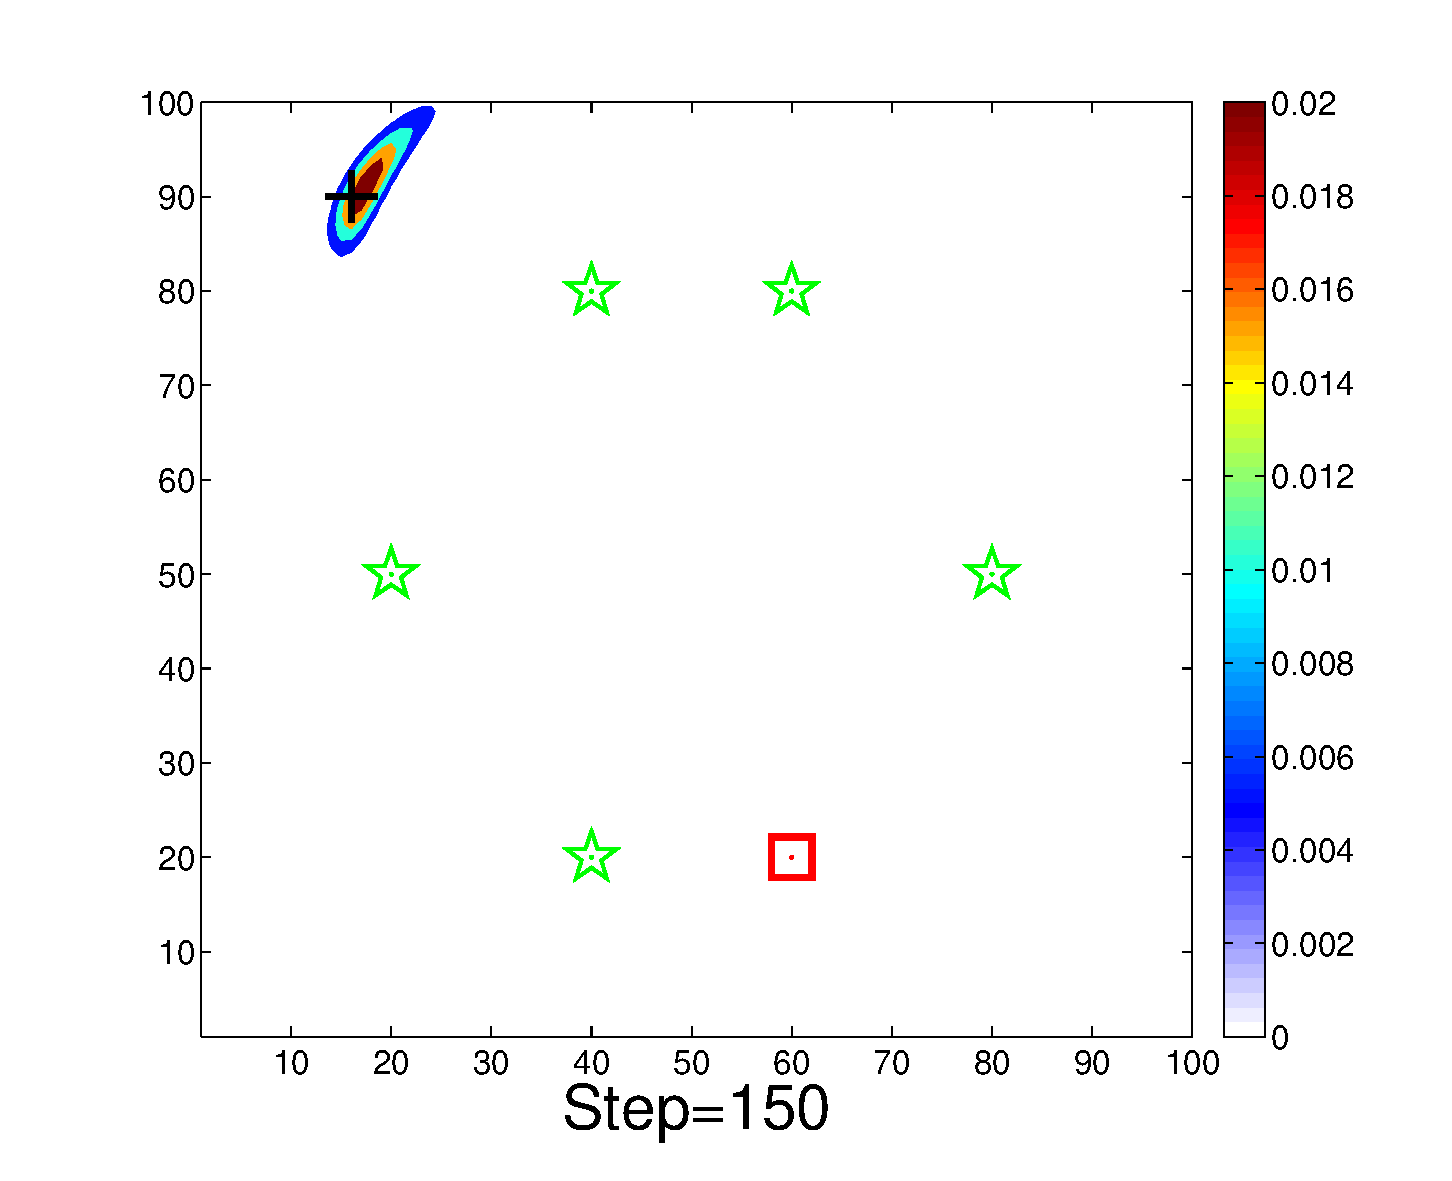
\includegraphics[width=\textwidth]{figures/sta_sen_sta_tar_top1_3_dbf_end}
%			\caption{\proto-DBF}\label{fig:sta_sen_sta_tar_top1_dbf}
%		\end{subfigure}
%		\begin{subfigure}[b]{0.21\textwidth}
%			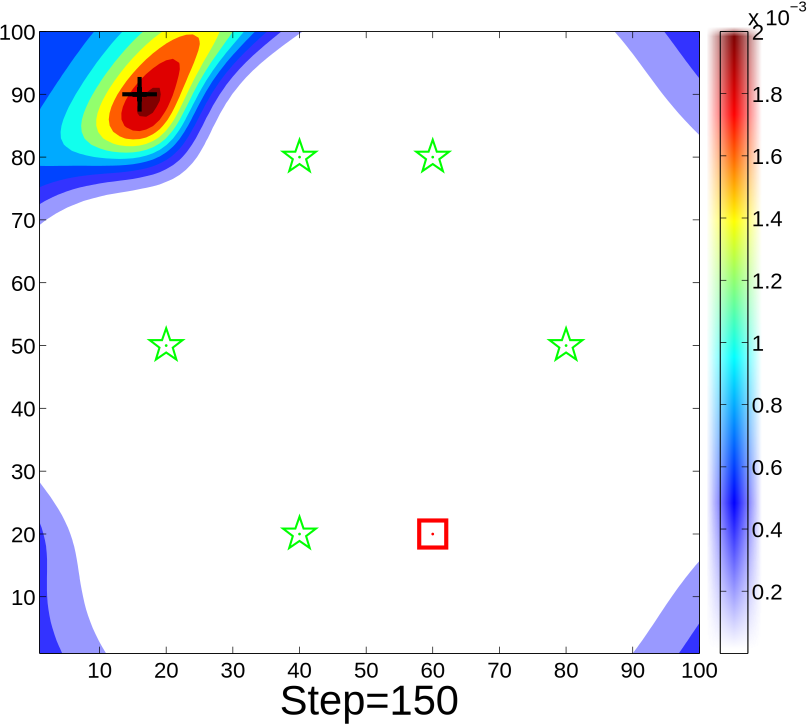
\includegraphics[width=\textwidth]{figures/sta_sen_sta_tar_top1_3_cons_end}
%			\caption{Consensus method}\label{fig:sta_sen_sta_tar_top1_cons}
%		\end{subfigure}
%		\begin{subfigure}[b]{0.21\textwidth}
%			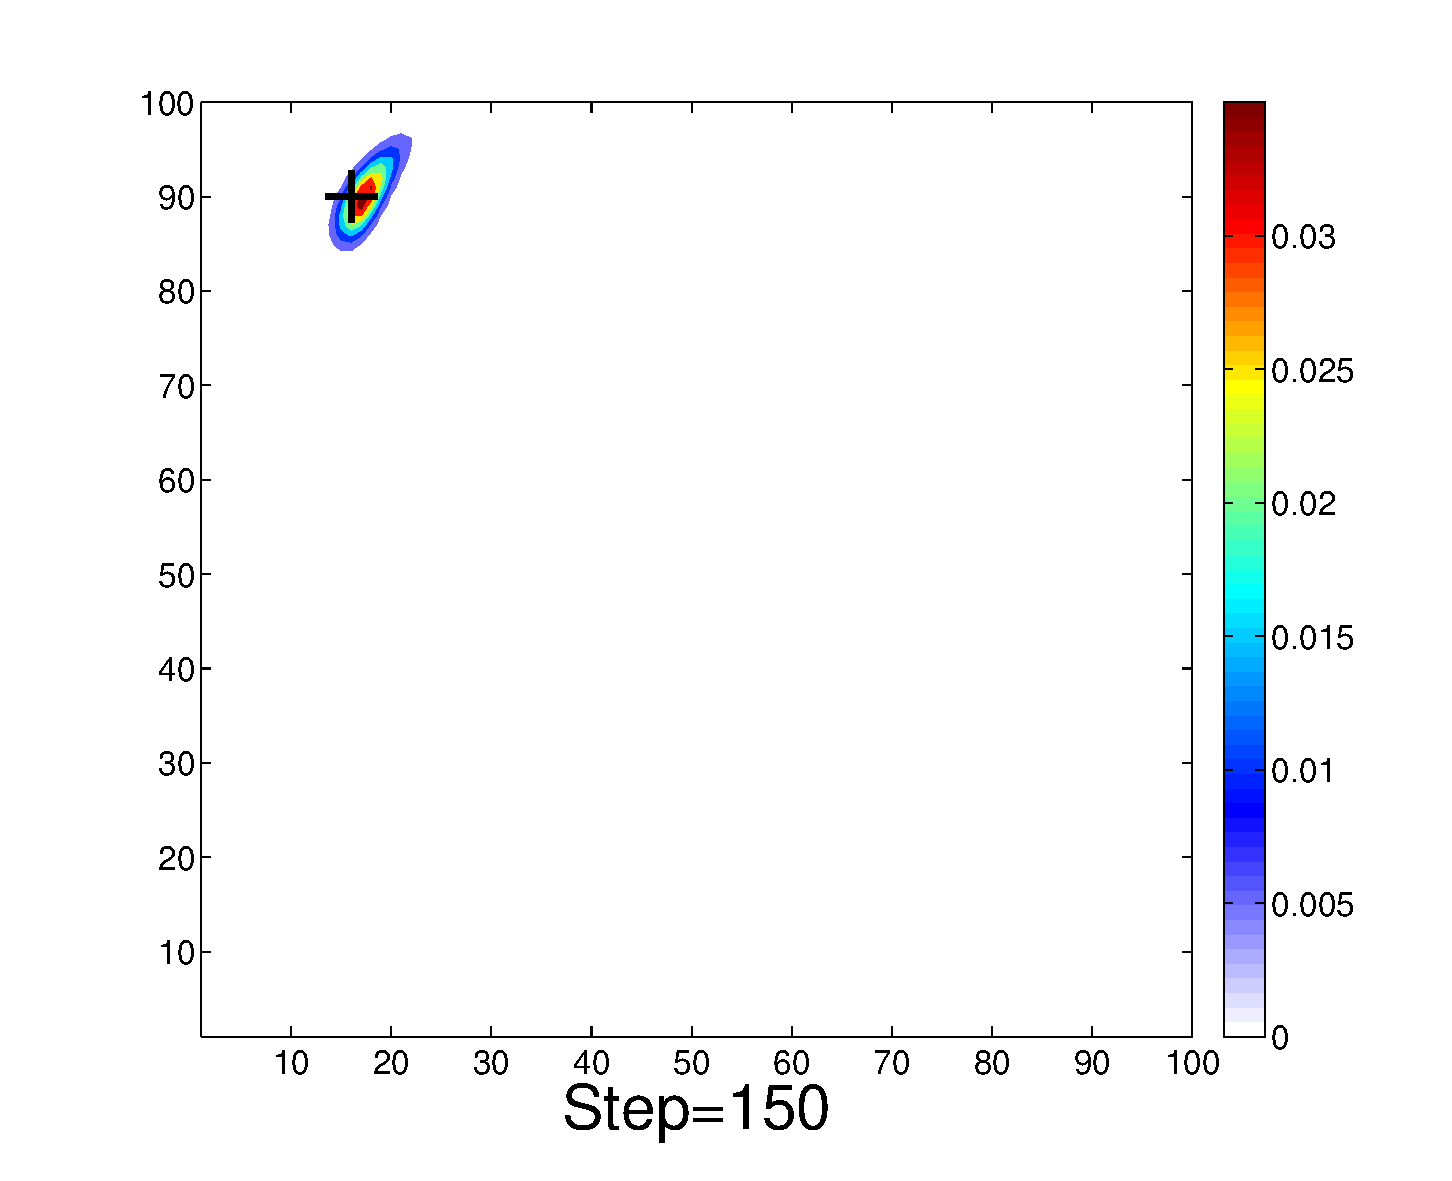
\includegraphics[width=\textwidth]{figures/sta_sen_sta_tar_top1_cent_end}
%			\caption{Centralized filter}\label{fig:sta_sen_sta_tar_top1_cent}
%		\end{subfigure}	
%		\begin{subfigure}[b]{0.23\textwidth}
%			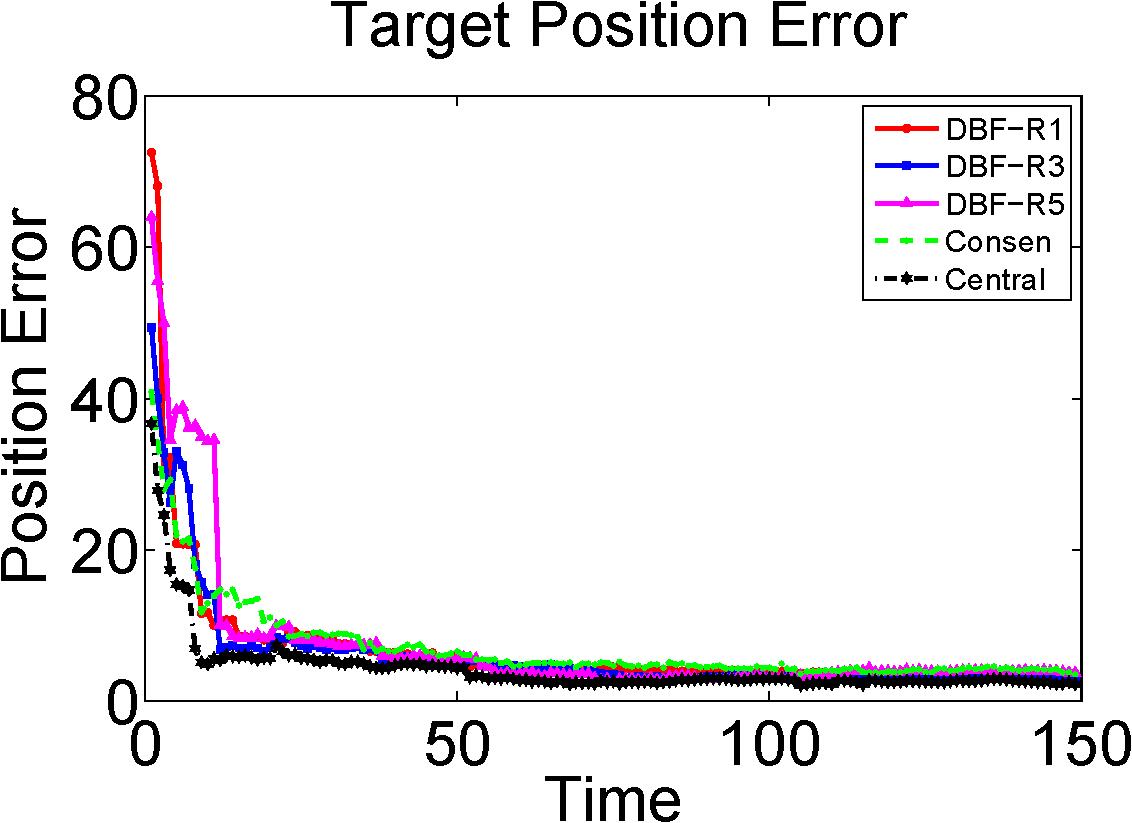
\includegraphics[width=\textwidth]{figures/sta_sen_sta_tar_top1_pos_err}
%			\caption{Position error}\label{fig:sta_sen_sta_tar_top1_pos_err}
%		\end{subfigure}	
%		\begin{subfigure}[b]{0.23\textwidth}
%			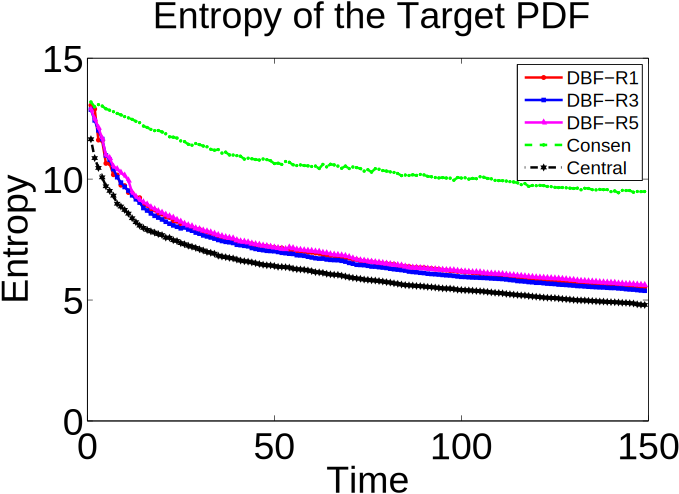
\includegraphics[width=\textwidth]{figures/sta_sen_sta_tar_top1_entropy}
%			\caption{Entropy reduction}\label{fig:sta_sen_sta_tar_top1_entropy}
%		\end{subfigure}		
%		\caption{First scenario: (a) two types of topologies; (b) individual PDF of the $3^\text{rd}$ UGV after initial observation; (c)-(e) PDFs at the end of simulation using different filters; (f) average position estimation errors; (g) average entropy of PDF. In last two figures, metrics are based on the PDFs of the $1^\text{st}$, $3^\text{rd}$ and $5\thi$ UGV using \proto-DBF, the common PDF using CbDF and using CF.}
%		\label{fig:sta_sen_sta_tar1}
%		\vspace{-1.3em}
%	\end{figure}
%	
%	In the first scenario, each UGV forms a circular individual PDF after the initial observation, centered at its own position, as shown in \cref{fig:sta_sen_sta_tar_top1_init_dbf}.
%	The circular PDF occurs because the sensor model only depends on the relative distance between a UGV and the target, not on the relative bearing.
%	As more observations are received by each UGV, the posterior individual PDF concentrates to the true location of the target (\cref{fig:sta_sen_sta_tar_top1_dbf}), which accords with the consistency of \proto-DBF.	
%	
%	Comparison of the estimation performance between \proto-DBF, CbDF and CF is presented in \cref{fig:sta_sen_sta_tar_top1_pos_err,fig:sta_sen_sta_tar_top1_entropy}.
%	Unsurprisingly, the CF achieves the best performance in terms of both small position estimation error and fast reduction of entropy. 
%	This happens because the central unit has access to the latest observations of all UGVs, thus making most use of all available information.
%	\proto-DBF and CbDF show similar performance as the CF does in position estimation error.
%	However, they significantly differ in terms of entropy reduction. 
%	In fact, \proto-DBF has similar asymptotic performance as the CF in reducing the entropy of PDF over time; this is notable since each UGV only communicates with its neighboring UGVs, which consumes less communication recourse than the CF.
%	The CbDF, on the contrary, is much slower in entropy reduction while incurring huge communication burden due to multiple rounds of consensus at each time step.
%	The difference in entropy reduction makes sense since CbDF can only ``implicitly" fuses different robots' observation via computing the average of individual PDFs while \proto-DBF and CF can directly utilize observations, thus making better use of available information.	
%	Such difference results in vastly different individual PDFs, as shown in \cref{fig:sta_sen_sta_tar_top1_dbf,fig:sta_sen_sta_tar_top1_cons,fig:sta_sen_sta_tar_top1_cent}, which show the PDF at the end of simulation.
%	Similar performance difference among \proto-DBF, CbDF and CF for the second scenario can be observed in \cref{fig:sta_sen_sta_tar2}.
%		
%	\begin{figure}%[thpb]
%		\centering
%		\begin{subfigure}[b]{0.45\textwidth}
%			
\includegraphics[width=\textwidth]{figures/com_topo2}
%			\caption{Collection of changing topologies}\label{fig:com_topo2}
%		\end{subfigure}
%		~
%		\begin{subfigure}[b]{0.21\textwidth}
%			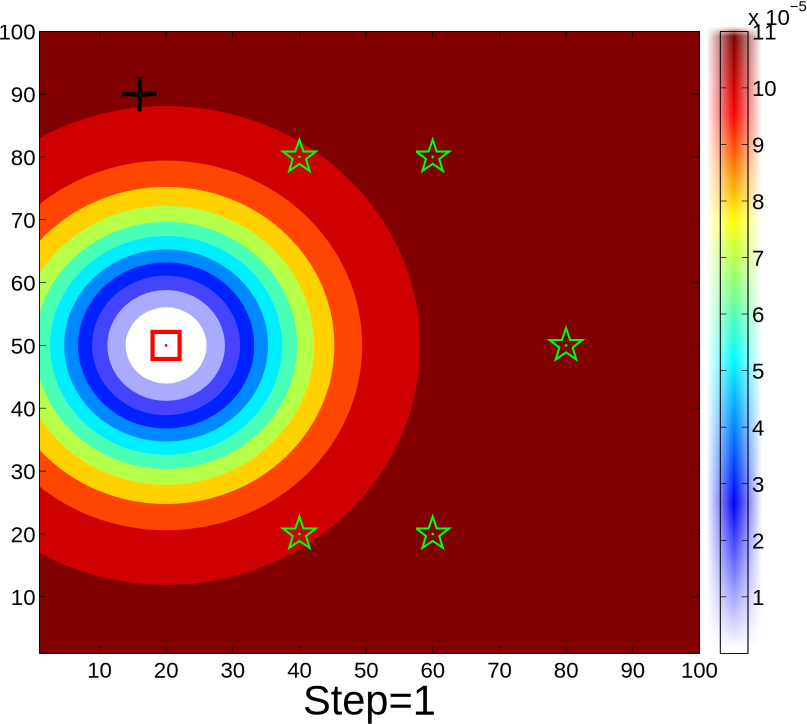
\includegraphics[width=\textwidth]{figures/sta_sen_sta_tar_top2_1_dbf_first}
%			\caption{Individual PDF}\label{fig:sta_sen_sta_tar_top2_init_dbf}
%		\end{subfigure}
%		\begin{subfigure}[b]{0.21\textwidth}
%			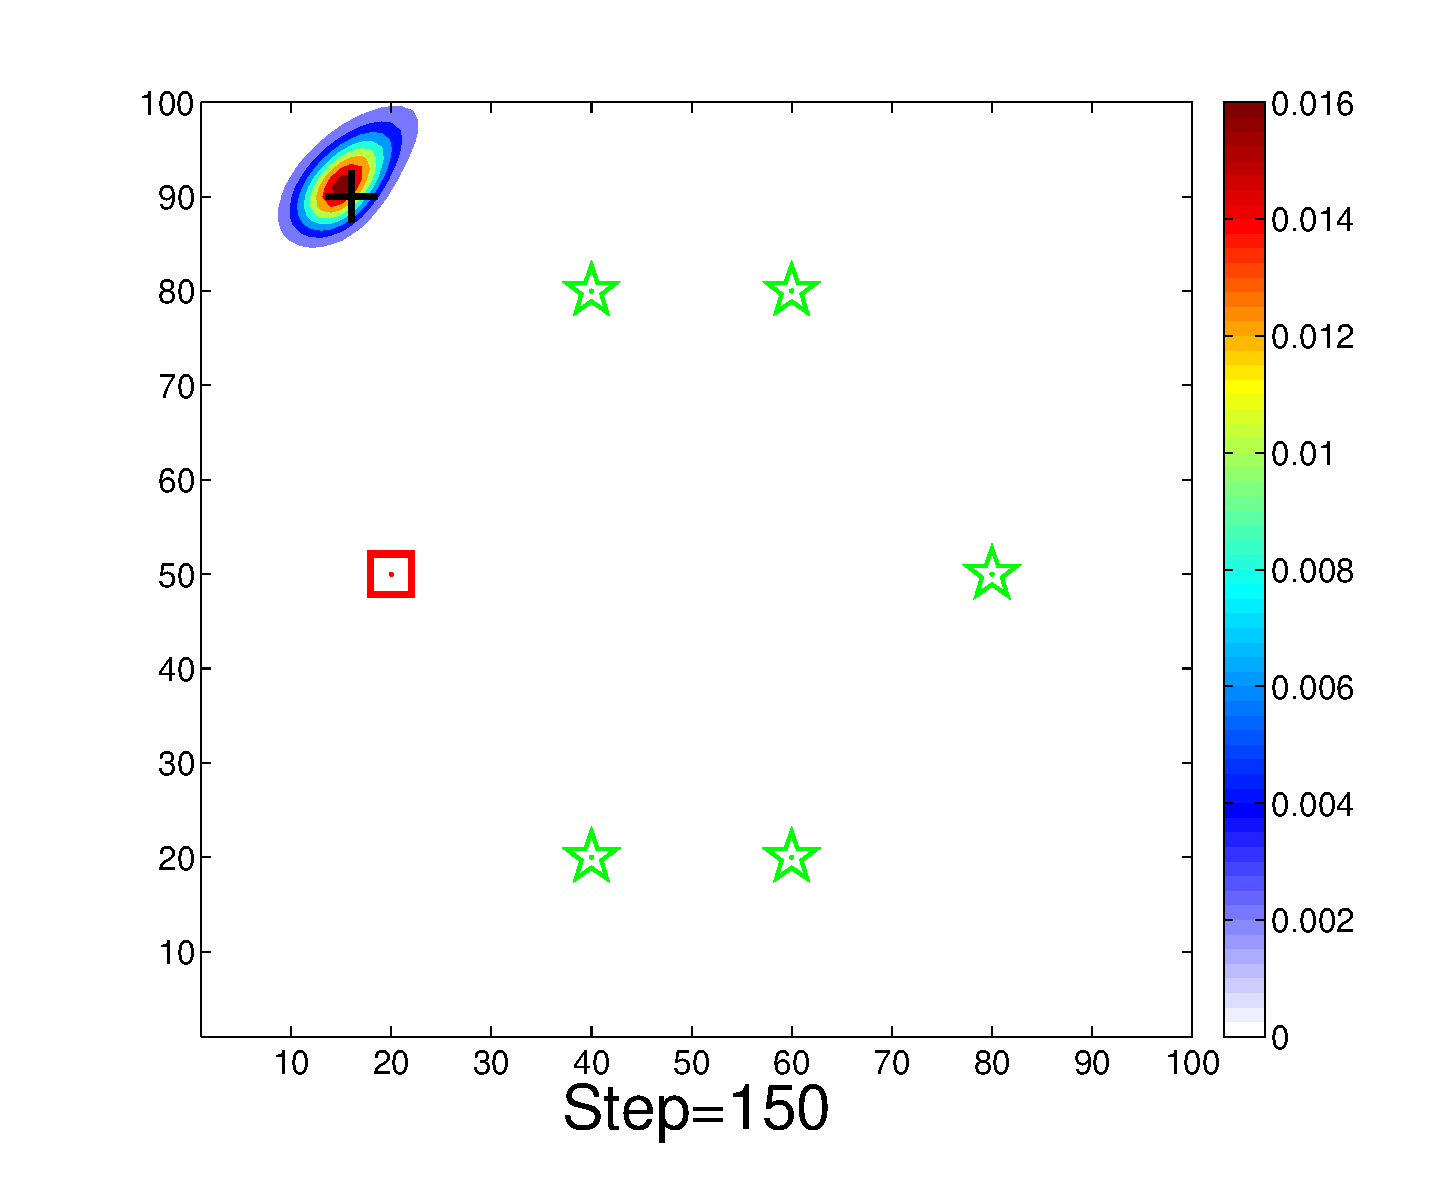
\includegraphics[width=\textwidth]{figures/sta_sen_sta_tar_top2_1_dbf_end}
%			\caption{\proto-DBF}\label{fig:sta_sen_sta_tar_top2_dbf}
%		\end{subfigure}
%		\begin{subfigure}[b]{0.21\textwidth}
%			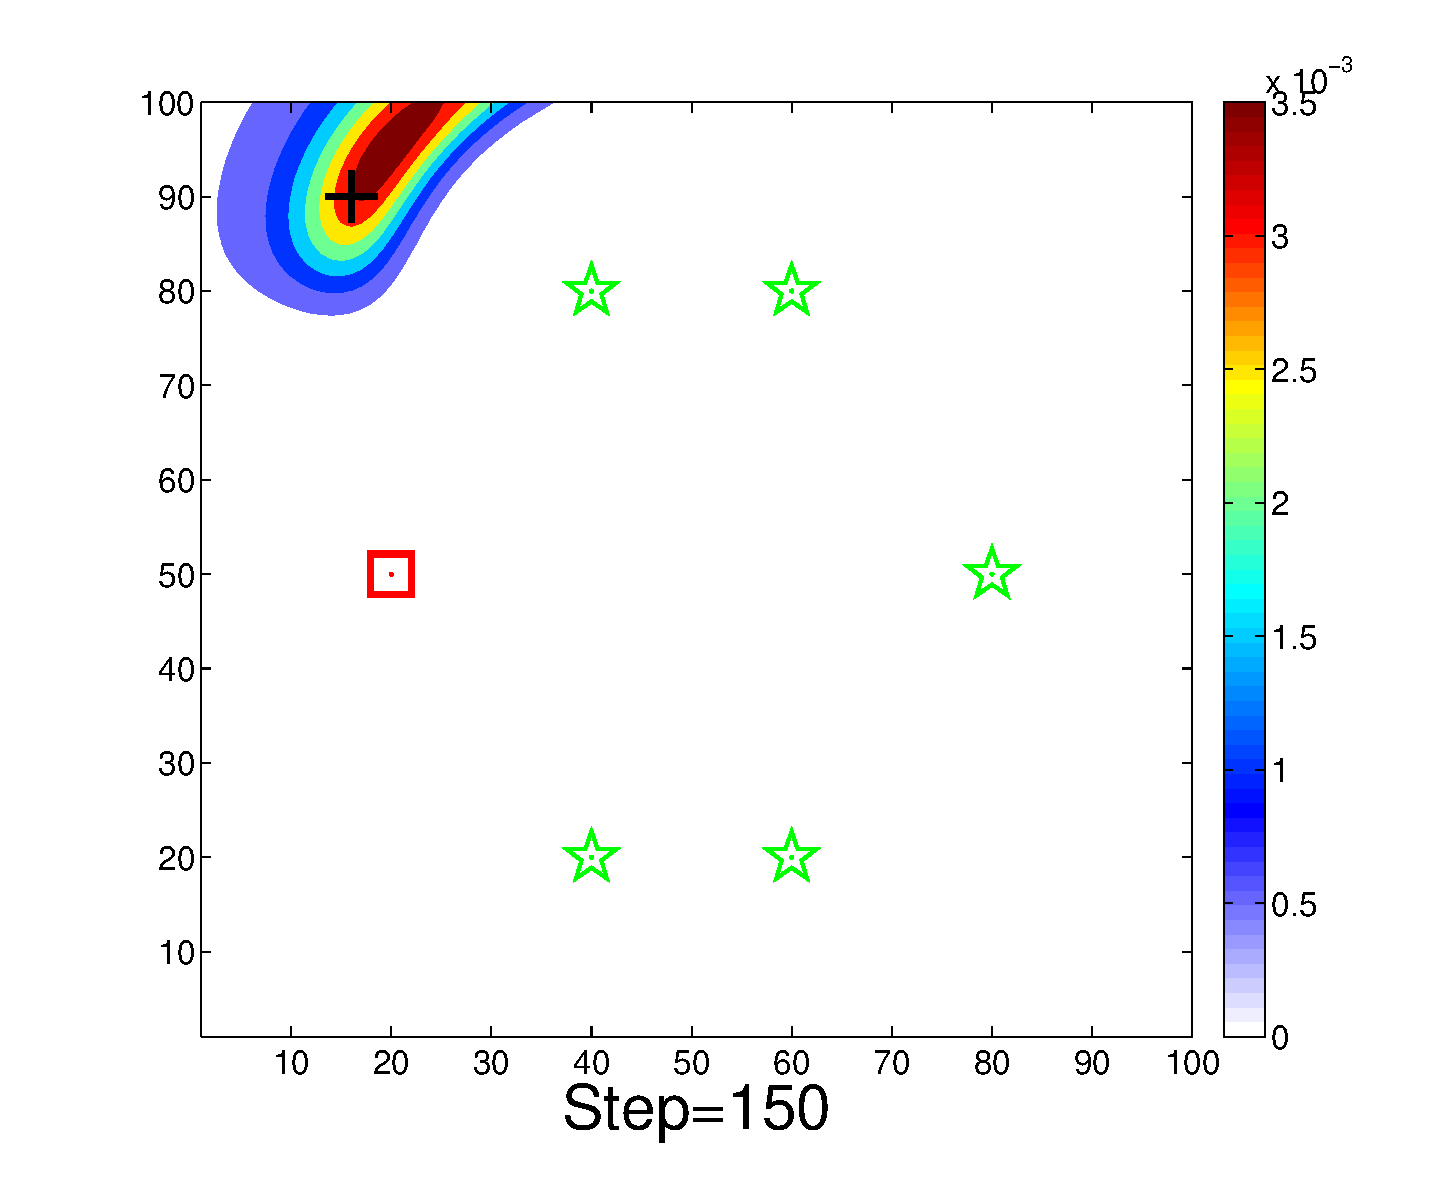
\includegraphics[width=\textwidth]{figures/sta_sen_sta_tar_top2_1_cons_end}
%			\caption{Consensus method}\label{fig:sta_sen_sta_tar_top2_cons}
%		\end{subfigure}
%		\begin{subfigure}[b]{0.21\textwidth}
%			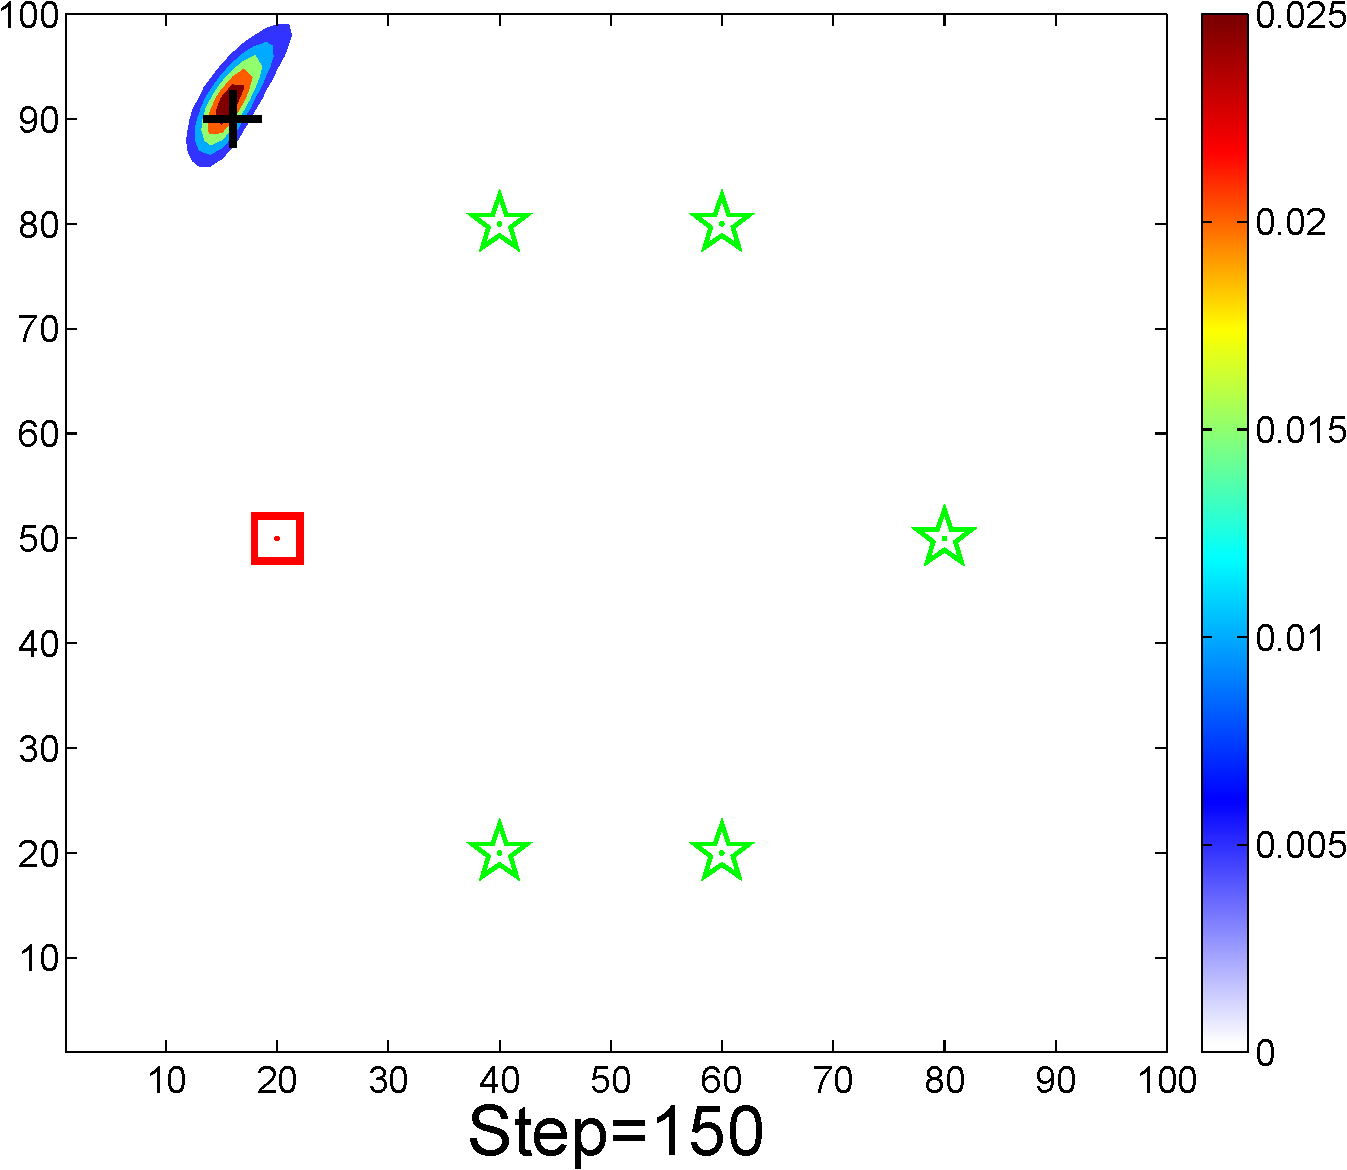
\includegraphics[width=\textwidth]{figures/sta_sen_sta_tar_top2_cent_end}
%			\caption{Centralized filter}\label{fig:sta_sen_sta_tar_top2_cent}
%		\end{subfigure}	
%		\begin{subfigure}[b]{0.23\textwidth}
%			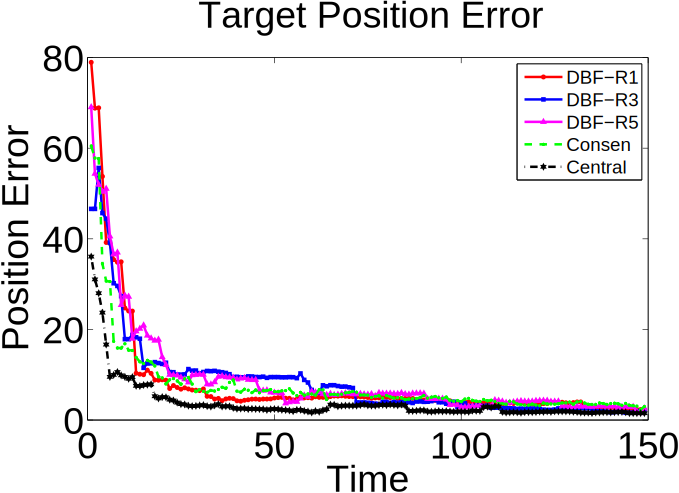
\includegraphics[width=\textwidth]{figures/sta_sen_sta_tar_top2_pos_err}
%			\caption{Position error}\label{fig:sta_sen_sta_tar_top2_pos_err}
%		\end{subfigure}	
%		\begin{subfigure}[b]{0.23\textwidth}
%			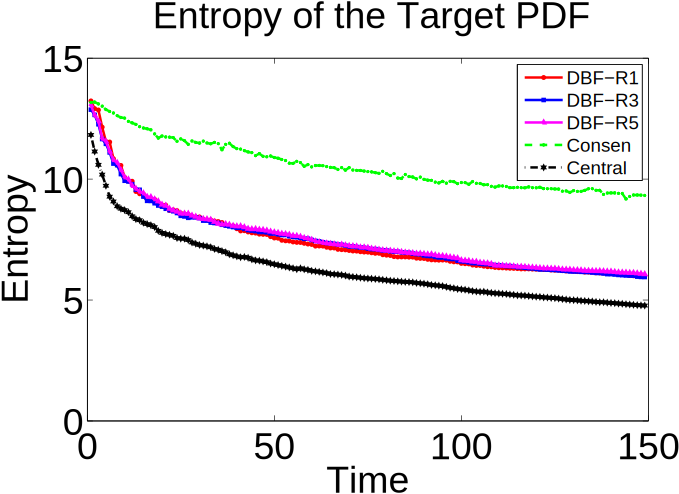
\includegraphics[width=\textwidth]{figures/sta_sen_sta_tar_top2_entropy}
%			\caption{Entropy reduction}\label{fig:sta_sen_sta_tar_top2_entropy}
%		\end{subfigure}		
%		\caption{Second scenario consists of three types of topologies. (b)-(d) show individual PDFs for $1^\text{st}$, $2^\text{nd}$ and $5\thi$ UGV, respectively.}
%		%			Individual PDFs for three switching interaction topologies: (b)-(e) The $1^\text{st}$ UGV's individual PDFs; (f)-(i) The $2^\text{nd}$ UGV's individual PDFs; (j)-(m) The $5^\text{nd}$ UGV's individual PDFs. }
%		\label{fig:sta_sen_sta_tar2}
%		\vspace{-1.3em}
%	\end{figure}
		